\documentclass[11pt,preprint, authoryear]{elsarticle}

\usepackage{lmodern}
%%%% My spacing
\usepackage{setspace}
\setstretch{1.2}
\DeclareMathSizes{12}{14}{10}{10}

% Wrap around which gives all figures included the [H] command, or places it "here". This can be tedious to code in Rmarkdown.
\usepackage{float}
\let\origfigure\figure
\let\endorigfigure\endfigure
\renewenvironment{figure}[1][2] {
    \expandafter\origfigure\expandafter[H]
} {
    \endorigfigure
}

\let\origtable\table
\let\endorigtable\endtable
\renewenvironment{table}[1][2] {
    \expandafter\origtable\expandafter[H]
} {
    \endorigtable
}


\usepackage{ifxetex,ifluatex}
\usepackage{fixltx2e} % provides \textsubscript
\ifnum 0\ifxetex 1\fi\ifluatex 1\fi=0 % if pdftex
  \usepackage[T1]{fontenc}
  \usepackage[utf8]{inputenc}
\else % if luatex or xelatex
  \ifxetex
    \usepackage{mathspec}
    \usepackage{xltxtra,xunicode}
  \else
    \usepackage{fontspec}
  \fi
  \defaultfontfeatures{Mapping=tex-text,Scale=MatchLowercase}
  \newcommand{\euro}{€}
\fi

\usepackage{amssymb, amsmath, amsthm, amsfonts}

\def\bibsection{\section*{References}} %%% Make "References" appear before bibliography


\usepackage[round]{natbib}

\usepackage{longtable}
\usepackage[margin=2.3cm,bottom=2cm,top=2.5cm, includefoot]{geometry}
\usepackage{fancyhdr}
\usepackage[bottom, hang, flushmargin]{footmisc}
\usepackage{graphicx}
\numberwithin{equation}{section}
\numberwithin{figure}{section}
\numberwithin{table}{section}
\setlength{\parindent}{0cm}
\setlength{\parskip}{1.3ex plus 0.5ex minus 0.3ex}
\usepackage{textcomp}
\renewcommand{\headrulewidth}{0.2pt}
\renewcommand{\footrulewidth}{0.3pt}

\usepackage{array}
\newcolumntype{x}[1]{>{\centering\arraybackslash\hspace{0pt}}p{#1}}

%%%%  Remove the "preprint submitted to" part. Don't worry about this either, it just looks better without it:
\makeatletter
\def\ps@pprintTitle{%
  \let\@oddhead\@empty
  \let\@evenhead\@empty
  \let\@oddfoot\@empty
  \let\@evenfoot\@oddfoot
}
\makeatother

 \def\tightlist{} % This allows for subbullets!

\usepackage{hyperref}
\hypersetup{breaklinks=true,
            bookmarks=true,
            colorlinks=true,
            citecolor=blue,
            urlcolor=blue,
            linkcolor=blue,
            pdfborder={0 0 0}}


% The following packages allow huxtable to work:
\usepackage{siunitx}
\usepackage{multirow}
\usepackage{hhline}
\usepackage{calc}
\usepackage{tabularx}
\usepackage{booktabs}
\usepackage{caption}


\newenvironment{columns}[1][]{}{}

\newenvironment{column}[1]{\begin{minipage}{#1}\ignorespaces}{%
\end{minipage}
\ifhmode\unskip\fi
\aftergroup\useignorespacesandallpars}

\def\useignorespacesandallpars#1\ignorespaces\fi{%
#1\fi\ignorespacesandallpars}

\makeatletter
\def\ignorespacesandallpars{%
  \@ifnextchar\par
    {\expandafter\ignorespacesandallpars\@gobble}%
    {}%
}
\makeatother

\newenvironment{CSLReferences}[2]{%
}

\urlstyle{same}  % don't use monospace font for urls
\setlength{\parindent}{0pt}
\setlength{\parskip}{6pt plus 2pt minus 1pt}
\setlength{\emergencystretch}{3em}  % prevent overfull lines
\setcounter{secnumdepth}{5}

%%% Use protect on footnotes to avoid problems with footnotes in titles
\let\rmarkdownfootnote\footnote%
\def\footnote{\protect\rmarkdownfootnote}
\IfFileExists{upquote.sty}{\usepackage{upquote}}{}

%%% Include extra packages specified by user

%%% Hard setting column skips for reports - this ensures greater consistency and control over the length settings in the document.
%% page layout
%% paragraphs
\setlength{\baselineskip}{12pt plus 0pt minus 0pt}
\setlength{\parskip}{12pt plus 0pt minus 0pt}
\setlength{\parindent}{0pt plus 0pt minus 0pt}
%% floats
\setlength{\floatsep}{12pt plus 0 pt minus 0pt}
\setlength{\textfloatsep}{20pt plus 0pt minus 0pt}
\setlength{\intextsep}{14pt plus 0pt minus 0pt}
\setlength{\dbltextfloatsep}{20pt plus 0pt minus 0pt}
\setlength{\dblfloatsep}{14pt plus 0pt minus 0pt}
%% maths
\setlength{\abovedisplayskip}{12pt plus 0pt minus 0pt}
\setlength{\belowdisplayskip}{12pt plus 0pt minus 0pt}
%% lists
\setlength{\topsep}{10pt plus 0pt minus 0pt}
\setlength{\partopsep}{3pt plus 0pt minus 0pt}
\setlength{\itemsep}{5pt plus 0pt minus 0pt}
\setlength{\labelsep}{8mm plus 0mm minus 0mm}
\setlength{\parsep}{\the\parskip}
\setlength{\listparindent}{\the\parindent}
%% verbatim
\setlength{\fboxsep}{5pt plus 0pt minus 0pt}



\begin{document}



\begin{frontmatter}  %

\title{Question 5: Volatility and GARCH estimates}

% Set to FALSE if wanting to remove title (for submission)




\author[Add1]{Gabriella Neilon}
\ead{22581340@sun.ac.za}





\address[Add1]{Stellenbosch University}

\cortext[cor]{Corresponding author: Gabriella Neilon}

\begin{abstract}
\small{
This analysis delves into the volatility of the Rand against select
currencies, aiming to compare South Africa's currency performance with
that of both developing and developed countries. Additionally, the study
investigates instances where the Rand demonstrates advantages,
particularly during periods of relative strength in the Dollar.
}
\end{abstract}

\vspace{1cm}





\vspace{0.5cm}

\end{frontmatter}

\setcounter{footnote}{0}



%________________________
% Header and Footers
%%%%%%%%%%%%%%%%%%%%%%%%%%%%%%%%%
\pagestyle{fancy}
\chead{}
\rhead{}
\lfoot{}
\rfoot{\footnotesize Page \thepage}
\lhead{}
%\rfoot{\footnotesize Page \thepage } % "e.g. Page 2"
\cfoot{}

%\setlength\headheight{30pt}
%%%%%%%%%%%%%%%%%%%%%%%%%%%%%%%%%
%________________________

\headsep 35pt % So that header does not go over title




\hypertarget{statement-1}{%
\section{Statement 1}\label{statement-1}}

The South African rand (ZAR) has over the past few years been one of the
most volatile currencies;

\begin{verbatim}
## Q(m) of squared series(LM test):  
## Test statistic:  1677.512  p-value:  0 
## Rank-based Test:  
## Test statistic:  3331.602  p-value:  0 
## Q_k(m) of squared series:  
## Test statistic:  8489.753  p-value:  0 
## Robust Test(5%) :  7435.948  p-value:  0
\end{verbatim}

\begin{verbatim}
## Sample mean of the returns:  7.22831e-06 0.000179327 0.0002452295 0.0002151889 1.978441e-05 
## Component:  1 
## Estimates:  0 0.033259 0.963705 
## se.coef  :  0 0.002579 0.002715 
## t-value  :  4.451156 12.89795 354.9005 
## Component:  2 
## Estimates:  0 0.085644 0.933416 
## se.coef  :  0 0.004219 0.002508 
## t-value  :  13.4003 20.30174 372.1938 
## Component:  3 
## Estimates:  3e-06 0.158857 0.783796 
## se.coef  :  0 0.010984 0.013002 
## t-value  :  13.64895 14.4619 60.28387 
## Component:  4 
## Estimates:  0 0.120259 0.888693 
## se.coef  :  0 0.007793 0.005987 
## t-value  :  7.933895 15.43177 148.4483 
## Component:  5 
## Estimates:  0 0.047263 0.943425 
## se.coef  :  0 0.004161 0.005244 
## t-value  :  4.964245 11.35975 179.8889
\end{verbatim}

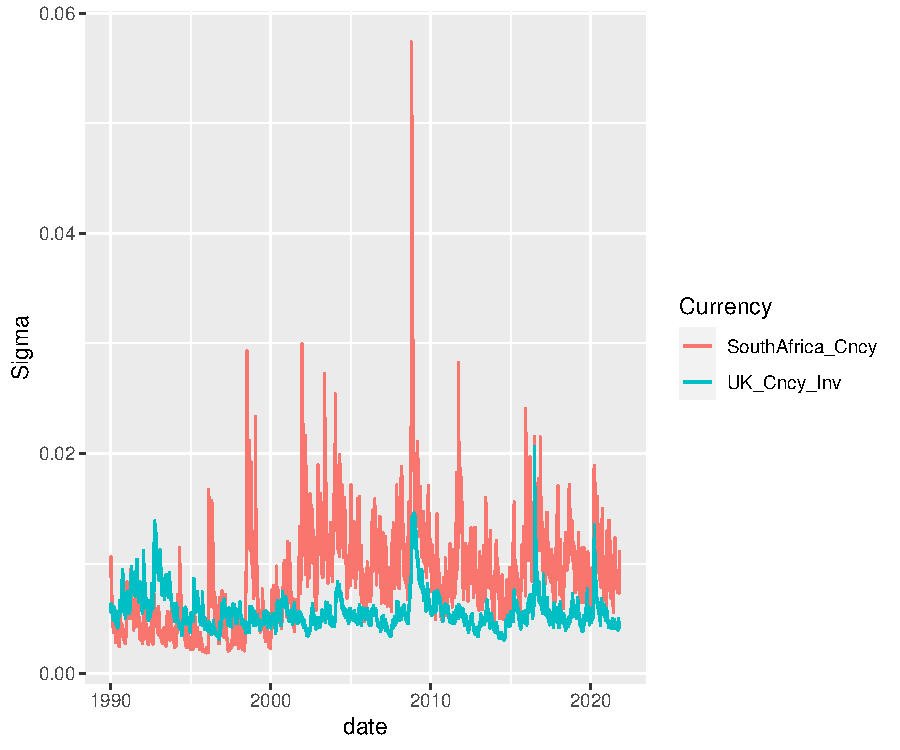
\includegraphics{Question-5_files/figure-latex/unnamed-chunk-2-1.pdf}

The MARCH test indicates that all the MV portmanteau tests reject the
null of no conditional heteroskedasticity, motivating our use of MVGARCH
models.

\hypertarget{statement-2}{%
\section{Statement 2:}\label{statement-2}}

The ZAR has generally performed well during periods where G10 currency
carry trades have been favourable and currency valuations relatively
cheap. Globally, it has been one of the currencies that most benefit
during periods where the Dollar is comparatively strong, indicating a
risk-on sentiment.

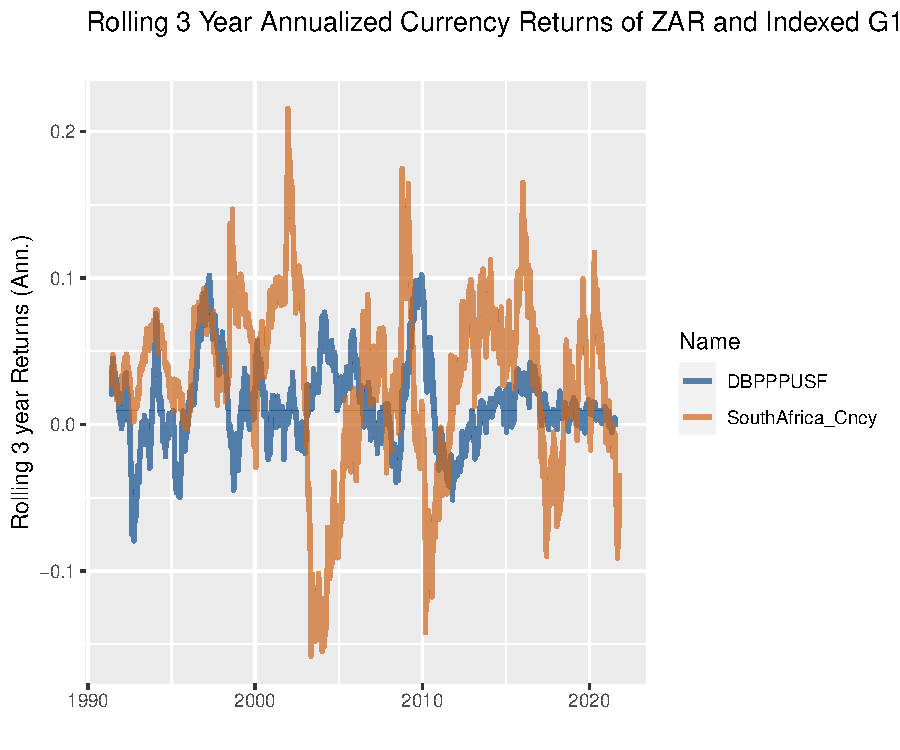
\includegraphics{Question-5_files/figure-latex/unnamed-chunk-3-1.pdf}

This figure illustrates a distinct relationship between the Dollar
(acting as the Carry Index) and the Rand; when the Dollar appreciates,
it tends to coincide with a subsequent depreciation in the Rand's value.
This relationship can be interpreted as a result of supply and demand
dynamics within these currencies. For instance, increased demand for the
Rand could drive its depreciation. This pattern suggests that when the
Dollar displays strength, the Rand appears relatively cheaper,
indicating an environment where there's heightened investment in the
Rand, typically reflecting a risk-on sentiment

\hypertarget{results}{%
\section{Results}\label{results}}

In periods of lowest flows, the top three funds---E473, N924,
R928---show an upward trend in returns, whereas the bottom three
funds---D394, T410, U411---indicate a downward trend. Conversely, during
periods of highest flows, the top three funds exhibit both upward and
downward trends in returns, while the bottom three funds showcase an
upward trend. Consequently, it appears that the fund performance does
not consistently align with the flow pattern, indicating that flow
volume might not serve as a reliable predictor of fund returns.

\hfill

\newpage

\bibliography{Tex/ref}





\end{document}
